\chapter{Lxc security}\label{features}

\textit{Linux Containers} achieve their execution environment security through the following concepts:\\
Chroot, namespaces, cgroups, privilege dropping, seccomp policies \cite{seccomp} and linux security modules
(e.g. \textit{AppArmor}\cite{apparmor} or \textit{SELinux}\cite{selinux}).\\
Seccomp policies are currently used by \textit{lxc} to blacklist some system calls that would modify the currently running kernel.\\
Linux security modules \cite{lsm} provide enhanced access control through the use of profiles which define application behaviour.\\
Neither seccomp policies nor any linux security module is used by this project.\\
Furthermore, most of the research has been done using \textit{Arch Linux} as the host OS which is why issues with its particular
kernel configuration are stressed explicitly.

\section{Chroot}\label{rootfs}

Using \textit{chroot} allows the caller to set a different directory as the new root directory.\\
The root of a filesystem is the point where all directory paths originate from.
Nothing exists in the virtual filesystem beyond this point. Typically a so called \textit{rootfs} contains all files needed for
the execution of a whole operating system.
The container rootfs is an exeption though because the kernel is already loaded by
the host system and is therefore not needed. Note that other \textit{chroot} environments do not need a kernel either but often have got one
since in many cases \textit{chroot} is used to install a new operating system on a machine.\\
\textit{Chroot} is not designed as a security feature and thus it is possible to break out of the current environment through
repeated invocation of the \texttt{chdir(``..'')} system call (see \cite{chrootbreak} for a complete example).\\
\textit{Lxc} uses the system call \texttt{pivot\_root} to change the root directory. This allows to unmount the host's rootfs after
successfully changing to the new root environment and therefore making sure that it has become inaccessible even through the hack
mentioned above.
By default the old rootfs is temporarily mounted in \texttt{/usr/lib/lxc/rootfs/lxc\_putold}. Directly after changing the environment successfully
it is unmounted \cite{pivotsetup}. Note that it is the default behaviour of \textit{lxc} to set up the namespaces before chrooting, so this
mountpoint will only exist in a new mount namespace (see chapter \ref{ns}).

\section{Namespaces}\label{ns}

Namespaces\cite{namespaces} are a feature of the \textit{linux} kernel. They allow to separate parts of the kernel from each
other which are traditionally global.
When spawning the container \textit{lxc} sets up the available namespaces which then separate the container from the host.\\
There are currently 6 namespaces in use by \textit{lxc}:\\
\textit{mnt} - The mount namespace separates mountpoints and filesystems.\\
\textit{pid} - The pid namespace creates separate environments each containing its own process hierarchy. Killing the process with PID 1
in a container for example will not affect the host's init process in any way but rather end the process inside the container with PID 1
(usually the container's own init process).\\
\textit{net} - The net namespace grants a separate network stack. The only device prevalent by default is a new instance of the loopback device.
To access any network
one must create a virtual ethernet device (veth) consisting of a pair of network devices, one in the original and one in the new namespace.\\
\textit{ipc} - The ipc (inter process communication) namespace prevents any interaction between processes in separate namespaces.\\
\textit{uts} - The uts namespace makes it possible to provide different information on the system such as the hostname, the OS name and version
when calling \texttt{uname}.\\
\textit{user} - The user namespace provides a mapping of user ids and group ids from the host's to the new namespace. A user may have the uid 0
(root) in the newly created namespace but uid 10000 in the host's namespace. So if this user ever manages to break the isolation of the
container, he will never be root on the host because his id is mapped to uid 10000.\\
In \textit{Arch Linux} and a few other distributions the user namespace is deactivated due to major concerns that this could open a broad
attack surface to unprivileged users \cite{archuserns}.

\section{Cgroups}

\textit{Cgroups} (control groups) is a kernel feature for limiting resources and access or simply supervising processes. The different cgroups exist as
pseudo filesystems in \texttt{/sys/fs/cgroup}. They are in general hierarchially organized: In each group subdirectories can be created
which inherit the settings of the parent control group. Settings are read and altered by reading from or respectively writing to the according
pseudofile. It is either possible to move an existing process to a cgroup by writing its PID into the \texttt{tasks} file present in each cgroup
or to use a tool like \textit{cgexec} provided with \textit{libcgroup}\cite{libcgroup} to execute a program directly in a cgroup.
Another common method is to launch a process from a parent process who is already in a cgroup. The child will then inherit the cgroups
from the parent.\\
These are the cgroups currently used in the config template for the \texttt{lxc\_daemon}:\\
\textit{cpu} - this cgroup is capable of setting priorities for CPU shares.\\
\textit{devices} - this cgroup allows or denies access to devices. \\
\textit{memory} - this cgroup is able to limit and provide information on memory resources.\\
The Fedora documentation features a full list of the prevalent cgroups \cite{cgroups}.

\section{Cgroup limits}

Cgroups is effective when it comes to limiting machine resources and as such preventing DoS attacks.
Also it is not -- except for the devices section -- preconfigured by \textit{lxc} in any way, so this needs some accounting:\\
It is crucial to limit the memory to prevent processes in the container from eating up the whole machine memory.
When the memory consumption reaches the specified threshold, the cgroups memory resource controller tries to reclaim memory first.
But if that fails, it will kill the most memory consuming process in the container which should result in a return code of 9\cite{cgrpmem}.
\text{Linux} does not write its data directly onto the hard disk but rather caches it for a certain amount of time to be able to
access it faster if this is required another time. Memory reclaim forces \textit{linux} to empty its IO cache.
This has been tested with a minimal C program which consumes as much memory as possible.\\
If the system has got swap memory this must also be limited. Otherwise it would just begin to swap out after the memory
threshold has been reached. Since the kernel does not distinguish between swapped or unswapped memory the limit should
be at least the same size as the memory limit.
Currently the \texttt{lxc\_daemon} does not determine whether the swap is activated or not. This needs to be adjusted manually in the cgroups
section of the config template by uncommenting the line stating \texttt{lxc.memory.msw.limit\_in\_bytes}.\\
Cgroups also provides a feature for limiting the CPU usage. It is possible to adjust the amount of CPU shares the process gets compared to
other processes on a scale from 1 to 1024. 256 is the current priority assigned to all containers run by the \texttt{lxc\_daemon}.
I have also provided a minimal CPU DoS C program which simply increments an integer in an infinite loop. Unfortunately this is hard to test
since the program still uses up the whole CPU capacity, it just gets a smaller portion compared to processes on default priority.\\
One of the severest DoS attacks is the fork bomb \cite{forkbomb}. Its only purpose is to replicate its process instance as much as possible until
the system freezes completely. Fortunately, cgroups provides
the \texttt{kmem} extension. The virtual memory is thoroughly divided between the userspace and the kernelspace\cite{kernelspace}.
It is essential that userspace programs
cannot modify any memory that the kernel uses as it would be very easy to forego any security feature -- or harm the system in any other possible way --
through simple memory modification. The process table which contains information about currently running processes is also part of the kernelspace,
so everytime the fork bomb creates a new instance this table grows in size.
The \texttt{kmem} extension is capable of limiting the kernel memory to a small amount. If set properly, this will cause the \texttt{fork}
system call to fail way before freezing the system. In conclusion after some trial-and-error-testing 12 MegaByte seems to be a
stable amount of allowed kernel memory.\\
Currently the \texttt{memory.kmem} feature is disabled in the default \textit{Arch Linux} kernel due to memory reclaim not being implemented yet\cite{kmembug}.\\

\section{Cgroup devices}

Another important cgroups feature is the device section.\\
A device is an interface between the userspace and the kernel for accessing hardware. It is identified by a major and a minor
device number.
The major device number specifies the device driver (e.g. SCSI for SATA hard drives) and the minor number refers to different
devices controlled by the same driver (e.g. partitions or terminals)\cite{devicenumbers}.\\
Furthermore, the kernel needs to be aware of the device type which is either block or character. This is due to different system
calls being used for each type.
The main difference between block and character devices is that block devices have a cache of their own and therefore are not
written or read directly upon like character devices.\\
First access to all devices is denied and then permitted exclusively.
%unfertig ... außerdem, wann passiert das?



\section{Capability dropping}\label{caps}

There are two types of users on a linux system: the root user who is basically allowed to do everything and the normal user 
who is not capable of performing any privileged operation. Kernel capabilities are a feature which allow a more distinct way of handling
permissions. In general the procedure is to start a program with root permissions and then dropping capabilities from the prevailing full set.
Any child process spawned will inherit this capability subset.
In some situations it might be more suitable to grant just a few capabilities while dropping the others, or maybe a program wants to do
privileged operations before handing the control over to some unstrustworthy program (which is the case with \textit{lxc}). Note
that unless CAP\_SETPCAP is dropped, the program can regrant itself any capability\cite{kernelcaps}.
As mentioned before lxc does not drop its capabilities immediately. The start processes as follows in a stripped down version (see figure \ref{figure_1}):\\
\begin{figure}[htb]
\begin{center}
  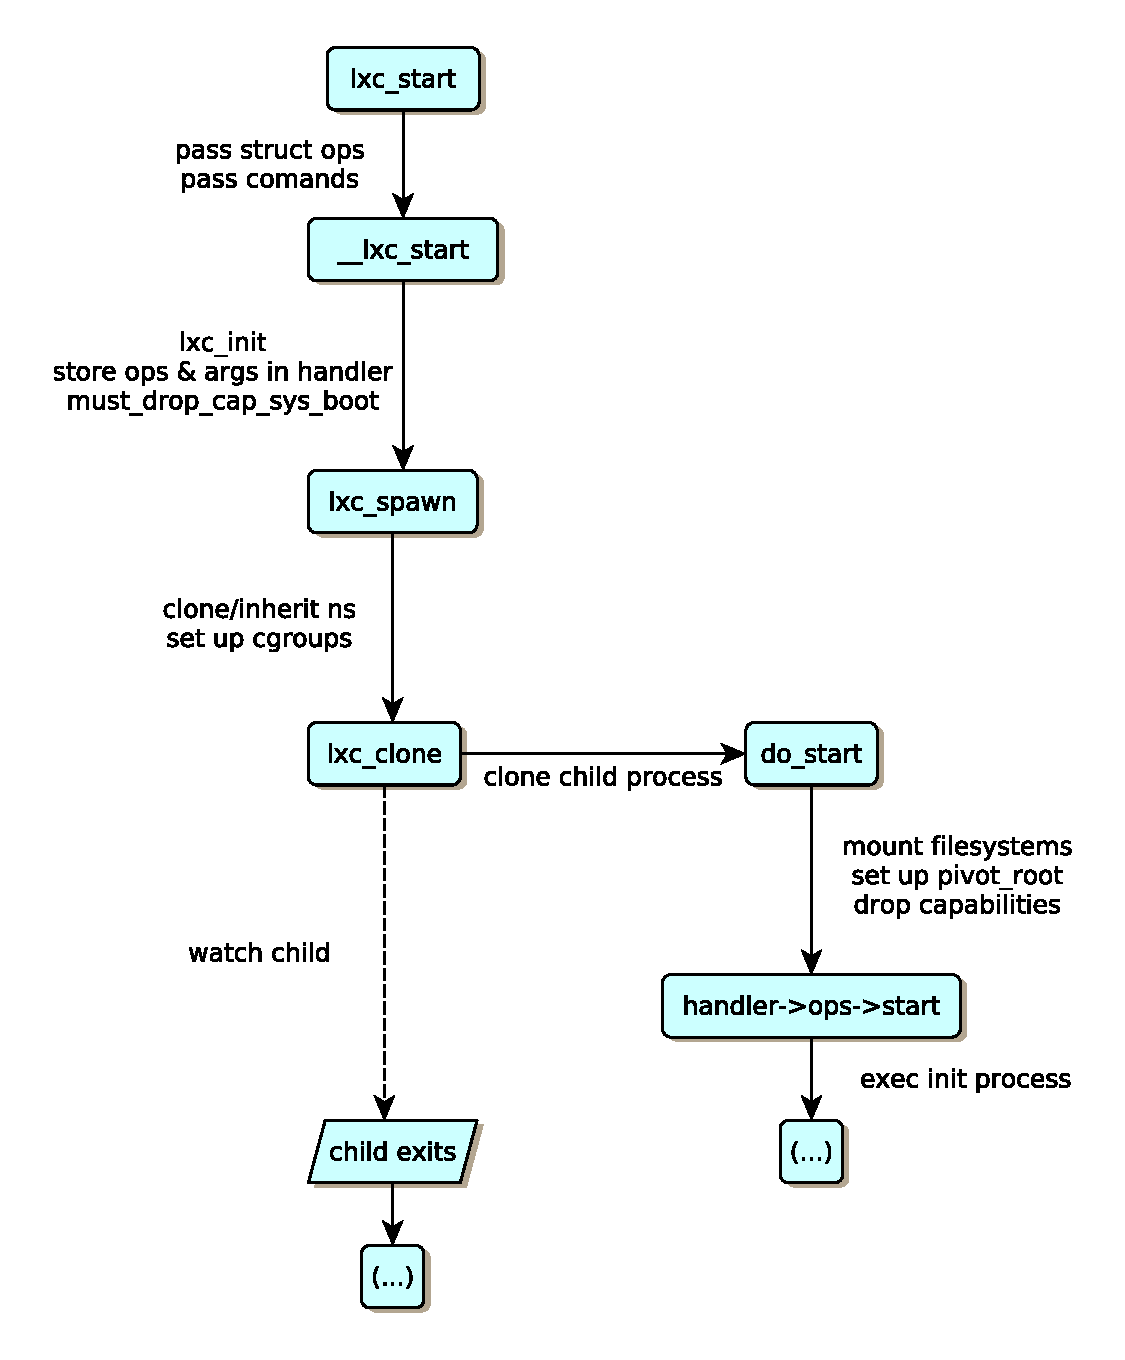
\includegraphics[width=300pt]{fig/figure_1.eps}
  \caption{start flowchart}
  \label{figure_1}
\end{center}
\end{figure}
Note that the nodes represent a ``step into'' exept for \textit{lxc\_clone --> child exits} which is a ``step over'' and -- as the parent is
irrelevant at this point for showing how capabilities are dropped -- does not point to another function but rather to a certain state.\\
In \texttt{\_\_lxc\_start} (start.c) the container first executes \texttt{lxc\_init} which mainly loads the seccomp policies (see chapter \ref{seccomp}),
sets the state to ``STARTING'' and environment variables for a pre-setup hook script. On return a \textit{handler} struct is handed to
\texttt{\_\_lxc\_start} which then adds the struct ops containing function references for later use and some commands given be the
initial caller (the first argument must be something like \texttt{/sbin/init}) to execute after lxc is done setting everything up for
the actual init process of the container.
Slightly afterwards \texttt{lxc\_spawn} is executed which then sets up cgroups according to the config specifications,
clones or inherits namespaces and creates a new process through \texttt{lxc\_clone}. This child process in turn executes \texttt{do\_start} which
mounts the filesystems accordingly and ultimately drops the privileges. After that it replaces itself with the init process of
the container through the \texttt{exec()} system call. The parent process waits for the child to complete its startup process and determines
if it simply exited or was signaled because it tried to do a reboot.\\
I have written a minimal c-program to test for capabilities inside the container which prints out every single one with
its label followed by the effective value, \texttt{1} for set \texttt{0} for unset. The code makes use of the shared library
\texttt{libcap.so.2}, so when running inside a container this must be present or else the test will fail.

\section{Mountpoints}

The only mounted filesystem besides the root filesystem is \texttt{/proc}. \texttt{/proc} is crucial for the execution environment because many
different programs rely on it to store and access process information.\\
The \texttt{/sys} filesystem contains amongst other things pseudofiles for accessing the machine hardware. As untrustworthy programs
having access to hardware settings is highly undesired, the safest yet most radical solution is not to mount \texttt{/sys}.